% Induction from a point stabiliser: constants and the sum-zero plane.
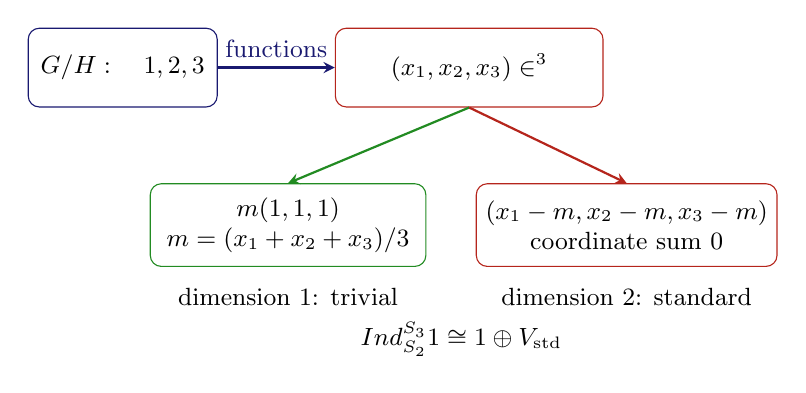
\begin{tikzpicture}[font=\small,>=stealth]
\node[draw=MidnightBlue,rounded corners,minimum width=2.4cm,minimum height=1.0cm] (cosets) at (0,0) {$G/H:\quad 1,2,3$};
\node[draw=BrickRed,rounded corners,minimum width=3.4cm,minimum height=1.0cm] (vectors) at (4.4,0) {$(x_1,x_2,x_3)\in\C^3$};
\draw[->,thick,MidnightBlue] (cosets) -- node[above] {functions} (vectors);
\node[draw=ForestGreen,rounded corners,align=center,minimum width=3.5cm,minimum height=1.05cm] (mean) at (2.1,-2) {$m(1,1,1)$\\$m=(x_1+x_2+x_3)/3$};
\node[draw=BrickRed,rounded corners,align=center,minimum width=3.8cm,minimum height=1.05cm] (plane) at (6.4,-2) {$(x_1-m,x_2-m,x_3-m)$\\coordinate sum $0$};
\draw[->,thick,ForestGreen] (vectors.south) -- (mean.north);
\draw[->,thick,BrickRed] (vectors.south) -- (plane.north);
\node[below=0.15cm] at (mean.south) {dimension $1$: trivial};
\node[below=0.15cm] at (plane.south) {dimension $2$: standard};
\node at (4.3,-3.45) {$\operatorname{Ind}_{\mathfrak S_2}^{\mathfrak S_3}1\cong 1\oplus V_{\mathrm{std}}$};
\end{tikzpicture}
